% ======================================================================================================
% TCC - César Henrique Bernabé
% Capítulo 2 - Referencial Teórico

% 
% ======================================================================================================
\chapter{Referencial Teórico}
\label{sec-referencial}

Este capítulo apresenta os principais conceitos teóricos que alicerçaram a evolução do metamodelo de requisitos do \zanshin e de conceitos que fundamentaram o desenvolvimento da ferramenta \unagi. A seção~\ref{sec-referencial-engenharia-objetivos} fala sobre Engenharia de Requisitos Orientada a Objetivos, destacando os principais conceitos dessa área que foram utilizados ao longo deste trabalho. A seção~\ref{sec-referencial-zanshin} apresenta o sistema \zanshin e os detalhes do metamodelo original do \framework. A seção~\ref{referencial-mdd} apresenta um breve resumo sobre Desenvolvimento Orientado a Modelos (\textit{Model Driven Development} ou MDD) assim como  as principais ferramentas que foram utilizadas durante o desenvolvimento do \unagi, como as funcionalidades \emf de modelagem do \eclipse, o plugin \sirius, dentre outros.

% ======================================================================================================
% SEÇÃO Engenharia de Requisitos Orientada a Objetivos
% ======================================================================================================

\section{Engenharia de Requisitos Orientada a Objetivos}
\label{sec-referencial-engenharia-objetivos}

% Engenharia de Software
A Egenharia de Software é uma área da Ciência da Computação voltada ao estudo dos processos, métodos, técnicas, ferramentas e ambientes de suporte ao desenvolvimento de software, apoiando-se principalmente nas práticas e aplicações da área de Gerência de Projetos com o objetivo de promover melhor organização, produtividade e qualidade em todo o processo de desenvolvimento de um software~\cite{falboEngSoft}.

% Engenharia de Requisitos
Dentro da área de Engenharia de Software, destaca-se uma importante subárea, a área de Egenharia de Requisitos de Software, focada no processo de elicitação de requisitos, considerados fatores determinantes no sucesso do desenvolvimento de um software~\cite{falboEngReq}. Requisitos podem ser entendidos como a definição do que o sistema pode prover, ou também entendidos como o que o sistema é capaz de fazer para atingir um determinado objetivo~\cite{pfleeger2004engenharia}.

% Objetivos
Devido ao fato de requisitos estarem diretamente ligados aos objetivos do sistema, destaca-se também a Engenharia de Requisitos Orientada a Objetivos, uma subárea da Engenharia de Requisitos. Objetivos são parte importante do processo de elicitação de requisitos, seu propósito é indicar as principais necessidades que justificam a criação de um determinado sistema, demonstrando os casos em que as funcionalidades do mesmo satisfarão as necessidades elicitadas, além de dizer como o sistema deve ser construído para satisfazê-las~\cite{ross1977structured}. 

Em uma descrição geral e resumida do processo de identificação de objetivos, pode-se dizer que o potencial software é analisado nos ambientes organizacional, operacional e técnico, onde são assim identificados os problemas de contexto e as oportunidades de solução desses problemas. Então, os objetivos são criados com foco na resolução dos problemas e das oportunidades identificadas. Tendo em mãos os objetivos do sistema devidamente refinados, os requisitos do sistema são então elaborados para que esses objetivos sejam devidamente atendidos. Além de apoiar no processo de modelagem de requisitos, objetivos são usados para apoiar outros propósitos como gerenciamento de conflitos e o processo de verificação~\cite{lapouchnian2005goal}. De acordo com~\cite{van2001goal}, objetivos podem ser reformulados em diferentes níveis de abstração dependendo do tipo de necessidade que o sistema alvo deve atender, abrangendo desde interesses referentes a estratégias de negócios até conceitos técnicos de atividades, assim referindo-se a requisitos funcionais e não-funcionais.

% Importancia Objetivos
A necessidade de uso de objetivos no processo de modelagem de sistemas de software vem se tornando cada vez mais clara a medida que analistas percebem que:
\begin{itemize}
	\item Objetivos provêm critérios claros de completude dos requisitos do sistema, permitindo também que requisitos desnecessários sejam descartados~\cite{van2001goal}.
	
	\item Objetivos facilitam o processo de entendimento dos requisitos pelas partes interessadas~\cite{van2001goal}.
	
	\item O uso de objetivos melhora a legibilidade de documentos de especificação de requisitos, pois permite que engenheiros possam enxergar com mais clareza as alternativas de desenvolvimento dos requisitos do sistema. Além de facilitar o processo de gerenciamento de conflitos~\cite{van2001goal}.
	
	\item Objetivos dirigem parte do processo de elicitação de requisitos, facilitando a identificação de boa parte deles~\cite{lapouchnian2005goal}.	
\end{itemize}

% Hardgoal, Softgoal, Quality Constraint e Domain Assumption
Diferentemente dos requisitos, objetivos podem precisar da cooperação entre diferentes tipos de refinamentos para que sejam atendidos de forma suficiente~\cite{dardenne1993goal}. Em outras palavras, um objetivo diretamente relacionado ao sistema a ser criado torna-se um Requisito, enquanto um objetivo sob responsabilidade de um agente do ambiente em que o software será executado torna-se uma Pressuposição de Domínio (ou \textit{Domain Assumptions}) e, nesse caso, são satisfeitos devido a uma regra de negócio~\cite{van2001goal, van1998managing}. Objetivos funcionais podem ser classificados como objetivos rígidos (\textit{Hard Goals}), cujo critério de satisfação pode ser atendido de forma técnica~\cite{dardenne1993goal} e objetivos fracos (\textit{Soft Goals}), que não possuem critérios claros de satisfação, entretanto são úteis quando deseja-se comparar os melhores refinamentos ao objetivo estudado. Para que \textit{Soft Goals} tenham um parâmetro claro de satisfabilidade, são adicionados a eles os Critérios de Qualidade (\textit{Quality Constraints}). Por exemplo, um \textit{Soft Goal} ``Baixo Custo'' pode ser refinado no critério de qualidade ``Custo deve ser menor que mil reais''. Por fim,~\cite{jureta2008revisiting} define outro tipo de refinamento para especificar a atendibilidade de um objetivo: as tarefas (\textit{Taks}), que são os passos a serem tomados para que um determinado objetivo seja cumprido. Em outras palavras, tarefas são definidas por funcionalidades do sistemas que, se executadas com sucesso, são consideradas satisfeitas~\cite{souza2012requirement}.

% Refinamentos
Objetivos relacionam-se um com o outro através de refinamentos. Segundo~\cite{dardenne1991goal, dardenne1993goal}, objetivos podem ser refinados usando grafos E/OU (\textit{AND/OR}). O critério de satisfabilidade de objetivos refinados em ``E'' ou ``OU'' segue os conceitos da lógica booleana: refinamentos do tipo ``E'' implicam que para que um objetivo seja considerado satisfeito, todos os sub-objetivos refinados a partir dele devem estar bem sucedidos, enquanto refinamentos do tipo ``OU'' relacionam o objetivo principal com um conjunto de alternativas, ou seja, basta que um de seus refinamentos seja atendido para que ele também seja considerado alcançado. Objetivos são refinados até atingirem um nível de granularidade em que são decompostos apenas por tarefas que podem ser completado com sucesso por um ator (humano ou outro sistema)~\cite{souza2013awareness}. Refinamentos podem acontecer entre Objetivos e outros Objetivos, \sofgoals, Tarefas e Pressuposições de Domínio.

%Representação Gráfica
Em questões de representação gráfica, os modelos de objetivos discutidos nesse texto são grafos ordenados que exibem as exigências das partes interessadas no topo do modelo e abaixo, objetivos (e tarefas) mais refinados, adotando uma topologia do tipo árvore. A simbologia utilizada é baseada na sintaxe de \istar~\cite{yu20111}. Um exemplo de modelo de objetivos representando um sistema de despacho de ambulâncias é mostrado na Figura~\ref{figura-acad-simples}.

\begin{figure}[h]
	\centering
	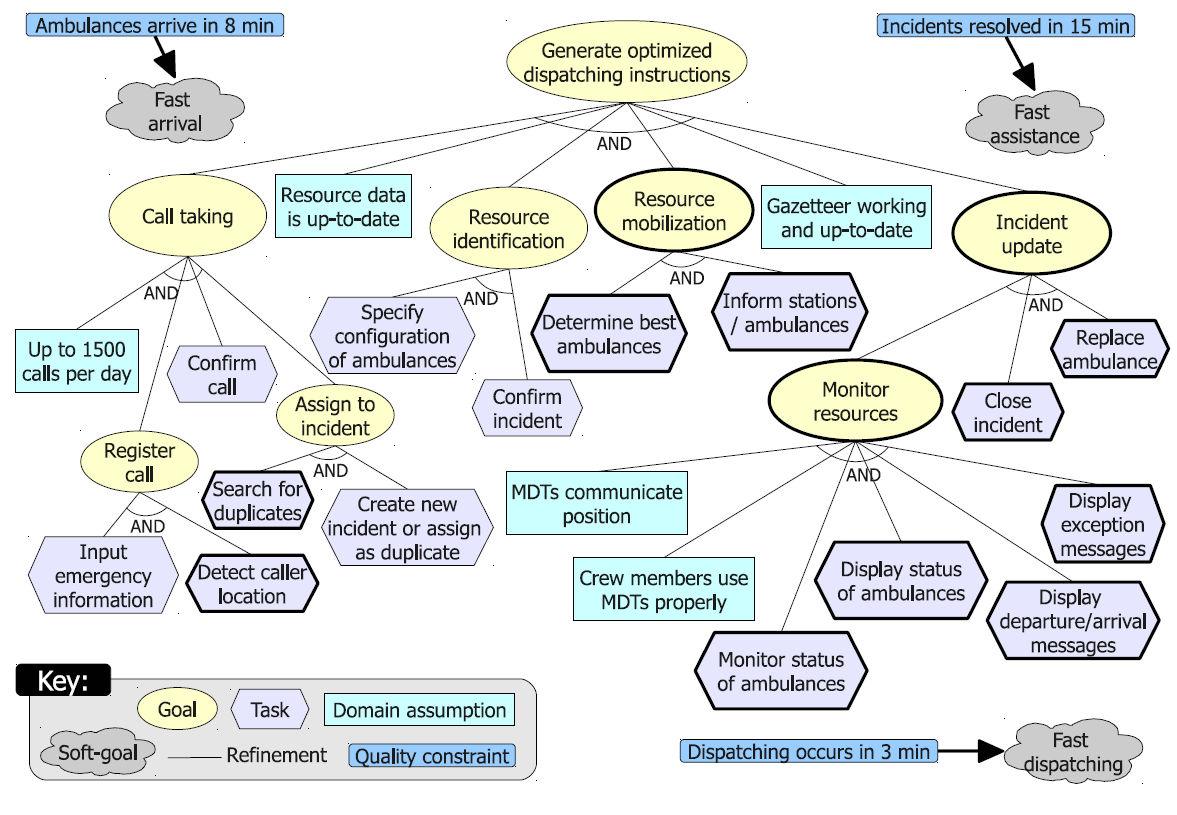
\includegraphics[width=1\textwidth]{figuras/modelos/ACAD-Simples.png}
	\caption{Exemplo de modelos de objetivos~\cite{tesevitor}}
	\label{figura-acad-simples}
\end{figure}

% ======================================================================================================
% SUBSEÇÃO Modelos de Objetivos em Tempo de Execução
% ======================================================================================================

\subsection{Modelos de Objetivos em Tempo de Execução}
\label{sec-referencial-engenharia-objetivos-runtime}

% Sistemas adaptativos
Muitas vezes os requisitos de um \textit{software} precisam ser modificados durante o ciclo de execução do mesmo. Além disso, ao longo do processo de especificação as partes interessadas no sistema podem apresentar requisitos condicionais, ou seja, que assumem diferentes configurações dependendo da ocorrência de determinada situação~\cite{souza2012requirement}. Em outras palavras, há a necessidade de sistemas que possam se automonitorar e, caso necessário, se adaptarem para que seus objetivos continuem sendo satisfeitos~\cite{dalpiaz2013runtime}. Esse tipo de sistema geralmente é composto por duas partes principais: a primeira sendo o sistema em si, que executa uma tarefa para cumprir um objetivo desejado e a segunda sendo um sistema de monitoramento do primeiro, que envia a ele instruções de modificação de suas configurações para que seus objetivos continuem sendo atendidos~\cite{souza2013awareness}. 

O sistema de monitoramento é construído fundamentado na premissa de que todo \textit{software} possui um ciclo de retroalimentação (\textit{feedback loop})~\cite{brun2009engineering}, e assim realizam o processo de adaptação com base nesse ciclo, aplicando controladores de resposta que monitoram o comportamento do sistema e injetam estratégias de adaptação~\cite{souza2013awareness}. O módulo adaptador verifica, de acordo com as saídas do sistema alvo, se os objetivos internos a esse estão sendo atendidos e, para isso, necessita importar o modelo de objetivos~\cite{souza2013awareness} enriquecido de elementos que indicam os requisitos a serem observados e as estratégias de adaptação relativas.

Modelos de sistemas adaptativos incluem requisitos autoconscientes, ou seja, definidos em relação ao sucesso, falha ou qualidade de serviço de outros requisitos~\cite{souza2013awareness}. Assim, esses são considerados ``requisitos especiais'', já que sua operacionalização está relacionada a mudança de outros requisitos~\cite{souza2012requirement}. Ademais, o comportamento do sistema é caracterizado por eventos que ocorrem em tempo de execução e que estão diretamente ligados a instâncias de objetivos~\cite{dalpiaz2013runtime}. Além disso, é importante observar que essa abordagem é considerada orientada a objetivos já que os requisitos mencionados são derivados do refinamento de objetivos elicitados para o sistema.

%Awreqs
Requisitos autoconscientes são divididos em dois tipos principais: Requisitos de Percepção (\textit{Awareness Requirements} ou \awreqs)~\cite{souza2013awareness} e Requisitos de Evolução (\textit{Evolution Requirements} ou \evoreqs)~\cite{souza2012requirement}. \awreqs são requisitos que referem-se ao estado de outros requisitos em tempo de execução, representando situações onde as partes interessadas desejam que o sistema se adapte~\cite{souza2012requirement}, e podem se referir a qualquer tipo de elemento, sejam objetivos, \sofgoals, tarefas e pressuposições de domínio. Ainda mais, \awreqs indicam o quão critico um requisito pode ser ao descrever o grau de tolerância a falhas do mesmo~\cite{souza2012requirement}. Antes da execução de um sistema, os requisitos estão em estado ``Não Decidido'' (\textit{Undecided}), e então pode assumir os estados ``Sucesso'' (\textit{Succeeded}), ``Falha'' (\textit{Failed}), e no caso de objetivos e tarefas, ``Cancelado'' (\textit{Canceled})~\cite{souza2013awareness}. É facilmente notável que o processo de elicitação de requisitos de percepção só acontece depois que o modelo de objetivos é levantado, e assim como o processo de construção de objetivos, \awreqs devem ser sistematicamente criados.

%Evoreqs
\evoreqs são requisitos que modificam o espaço de comportamento do sistema, permitindo que novas alternativas de requisitos sejam usadas, baseando-se em um conjunto pré-definido de etapas de evolução para os requisitos monitorados~\cite{souza2012requirement}. Isto é, \evoreqs são requisitos que especificam uma série de operações primárias em relação a outros requisitos diante de determinadas situações, dizendo ao sistema como adaptar-se~\cite{souza2012requirement}, como por exemplo, instruções para adicionar, remover ou modificar o estado de um objetivo (em nível de instância), desfazer as ações de uma execução que resultou em falha, entre outras~\cite{souza2013requirements}.

Em suma, \awreqs especificam quando um determinado objetivo precisa de mudanças para continuar a ser atendido, enquanto \evoreqs especificam como executar tais mudanças. A seguir, o modelo de exemplo apresentado na seção~\ref{sec-referencial-engenharia-objetivos} é novamente apresentado, porém com novos requisitos de adaptação que são devidamente discutidos na próxima sessão.

% ======================================================================================================
% SUBSEÇÃO Exemplo de Caso de Uso
% ======================================================================================================
\subsection{Exemplo de Modelagem de Caso de Uso}
\label{sec-referencial-engenharia-objetivos-exemplo}

Na Figura~\ref{figura-acad-completo} é apresentado o modelo visual completo do sistema de despacho de ambulâncias (\textit{Adaptive Computer-aided Ambulance Dispatch} ou \textit{A-CAD}), nele observa-se o objetivo principal ``Gerar Instruções de Despacho Otimizadas'', representado por uma oval, que é imediatamente refinado em outros objetivos e em uma pressuposição de domínio (retângulo). O refinamento entre o objetivo raiz e seus filhos imediatos é do tipo ``E'' e portanto, para que o objetivo principal seja considerado satisfeito, todos as suas decomposições de primeiro grau precisam ser satisfeitas. Então, verifica-se que o primeiro nível de refinamento do objetivo principal é composto dos objetivos ``Gerenciar Chamadas'', ``Identificação de Recursos'', ``Mobilização de Recursos'', ``Obtenção de Mapas''e da pressuposição de domínio ``Dados sobre recursos está sempre atualizado''.

\begin{figure}[h]
	\centering
	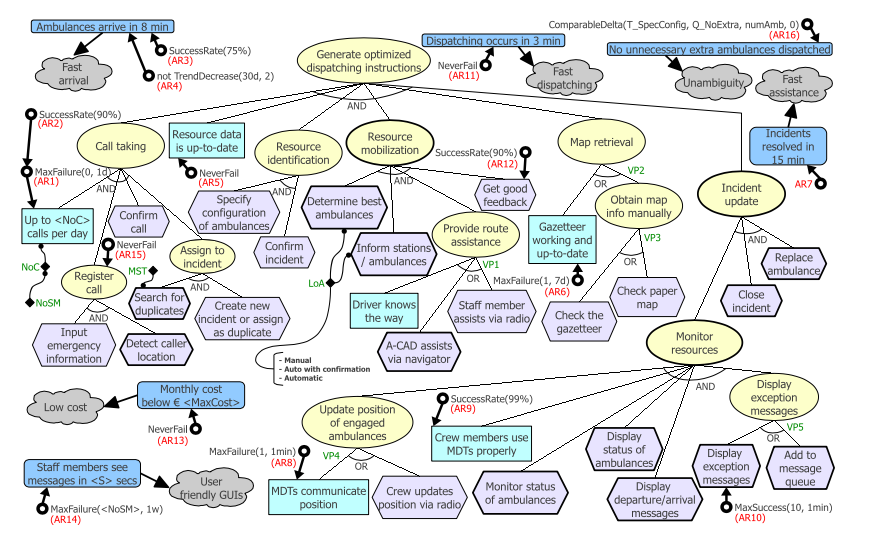
\includegraphics[width=1\textwidth]{figuras/modelos/ACAD-Completo.png}
	\caption{Exemplo de modelos de objetivos de um sistema de despacho de ambulâncias ~\cite{tesevitor}}
	\label{figura-acad-completo}
\end{figure}

O processo de refinamento do modelo então segue até que todos os objetivos sejam completamente decompostos em tarefas ou pressuposições de domínio. \sofgoals são simbolizados por nuvens e refinados em critérios de operacionalização representados por retângulos com cantos arredondados. Exemplificando, o \sofgoal ``Chegada Rápida'' é operacionalizado por ``Ambulâncias chegam em oito minutos'', assim, tem-se um critério claro de satisfação para um objetivo que antes possuía diversos tipos de interpretação, porém agora, sabe-se que uma ambulância chega rapidamente se consegue estar no local do acidente em menos de oito minutos a partir da chamada.

Os requisitos de percepção são representados por um círculo oco. Por exemplo, o \awreq identificado por ``AR15'', indica que o objetivo ``Registrar Chamados'' deve ``Nunca falhar'' (\texttt{NeverFail}). Os \evoreqs referentes a cada um dos \awreqs não são representados nesse modelo, e devem ser especificados em forma de sequencia de operações sobre os elementos do modelo de objetivos (essa escolha visa aprimorar a legibilidade do modelo). Além dos \awreqs, são especificados também os parâmetros de controle (\textit{Control Parameters}), representados por losangos, que indicam parâmetros do sistema que podem ser reconfigurados durante a adaptação. Todas as formas de representação estão resumidas na Figura~\ref{figura-elementos-gore-eca}.

\begin{figure}[h]
	\centering
	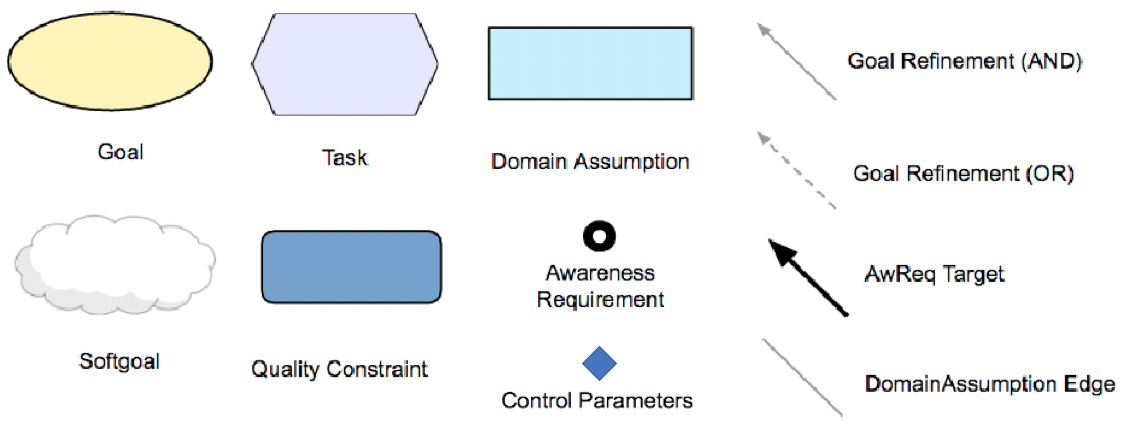
\includegraphics[width=1\textwidth]{figuras/modelos/Elementos-GORE.png}
	\caption{Representação gráfica de elementos de \gore}
	\label{figura-elementos-gore-eca}
\end{figure}

Sobre os \evoreqs do ``AR15'', podemos definir seus respectivos Requisitos de Evolução. Primeiramente, se o objetivo vir a falhar, define-se a primeira estratégia de adaptação como ``Tentar Novamente em 5 segundos no máximo uma vez'' (\texttt{RetryStrategy(5000)}), caso falhe mais do que uma vez, aplica-se outra estratégia ``Diminuir Condições ao Desabilitar Filho'' (\texttt{RelaxDisableChild(TDetectCaller)}), que desativa o requisito ``Detectar Localização da Ligação'', também aplicado no máximo uma vez. Essas decisões são sumarizadas na tabela \ref{tabela-evoreqs-ar15}.

\begin{table}[]
	\centering
	\caption{Tabela de especificação das estratégias de adaptação de AR15.}
	\label{tabela-evoreqs-ar15}
	\begin{tabular}{lll}
		\cline{1-3}
		\multicolumn{1}{|l|}{AR15} & \multicolumn{1}{l|}{NeverFail(G\_RegCall)} & \multicolumn{1}{l|}{\begin{tabular}[c]{@{}l@{}}1. Retry(5000)\\ 2. RelaxDisableChild(T DetectCaller)\end{tabular}} \cline{1-3}
	\end{tabular}
\end{table}

O processo de especificação de como as estratégias de evolução são realizadas pelo sistema é discutido na próxima seção.

% ======================================================================================================
% SEÇÃO Zanshin
% ======================================================================================================

\section{Zanshin}
\label{sec-referencial-zanshin}

Apresentado por~\cite{tesevitor}, \zanshin é um \textit{framework} que utiliza de ciclos de retro-alimentação para monitorar sistemas e enviar estratégias de adaptação com base em informações de modelos de requisitos orientados a objetivos enriquecidos com elementos como os \awreqs e os \evoreqs. O nome \zanshin vem de um termo usado em artes marciais japonesas e significa estado de completa consciência.

Em tempo de execução, os elementos do modelo de objetivos são representados por classes e instanciados cada vez que o usuário (ou sistema) busca atingir um objetivo, e então o sistema passa a enviar mensagens a essas instâncias quando detectar falhas. Percebe-se assim, que objetivos e pressuposições de domínio não são tratadas como invariantes que devem sempre ser atingidas, já que o sistema pode falhar ao tentar atingir seus objetivos iniciais, e então o componente de adaptação lidará com essas falhas e tomará medidas para que os objetivos voltem a ser satisfeitos~\cite{souza2013requirements}.

Assim como o monitoramento de objetivos através do \textit{Feddback Loop}, o \zanshin também monitora Parâmetros (\textit{Parameters}) que podem ser definidos em dois tipos. Primeiro, os Pontos de Variação (ou \textit{Variation Points}), que representam refinamentos do tipo ``OU'' (\textit{OR}). Por exemplo, o VP4 do modelo de objetivos do sistema A-CAD (Figura~\ref{figura-acad-completo}) que refere-se ao objetivo ``Atualizar posição de ambulâncias em uso'' especifica que atualizações de posição das ambulâncias podem ser obtidas automaticamente ou via rádio. Segundo, as Variáveis de Controle (ou \textit{Control Variables}), que são abstrações referentes a pontos de variação repetitivos ou usados em grande escala, como por exemplo a variável MST (``Tempo de Busca Mínimo'' ou \textit{Minimum Search Time}), que refere-se a tarefa ``Procurar por (incidentes) duplicados''. A especificação do comportamento dessas estratégias é discutido em seções posteriores.

O metamodelo dos modelos de objetivos usados no \zanshin é representado na Figura~\ref{figura-metamodelo-antigo}, e especificado no código do \textit{framework} como um modelo \ecore e carregado em memória como objetos \java usando um \framework do \eclipse conhecida como \textit{Eclipse Modeling Framework}. Nessa caso, o modelo \ecore representa os tipos de requisitos em nível de classe~\cite{souza2013requirements}. 

\begin{figure}[h]
	\centering
	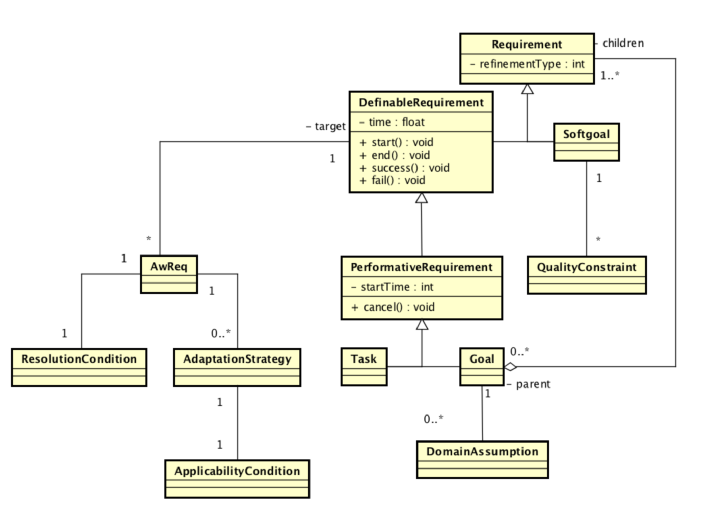
\includegraphics[width=1\textwidth]{figuras/metamodelos/metamodelo-zanshin-antigo.png}
	\caption{Metamodelo que define a sintaxe abstrata para o \zanshin}
	\label{figura-metamodelo-antigo}
\end{figure}

O \zanshin é ser divido em quatro componentes principais, entretanto essa seção discute desses: o componente de monitoramento e o componente de adaptação.

% ======================================================================================================
% SUBSEÇÃO Zanshin: Monitoramento
% ======================================================================================================
\subsection{Monitoramento}
\label{sec-referencial-zanshin-monitoramento}

O módulo de monitoramento necessita que o sistema alvo implemente funcionalidades de registro (\textit{logs}). Através do registro, o sistema pode detectar mudanças nos estados das instâncias de um \awreq e assim notificar o serviço de adaptação sobre essas ocorrências. 

Para identificar o modelo de objetivos do sistema alvo, o componente de monitoramento necessita da especificação do modelo do domínio também em \ecore. Através dele, o \zanshin criará instancias desses objetivos estendendo as classes carregadas do metamodelo de \gore referentes ao tipo de cada um deles (Figura~\ref{figura-metamodelo-antigo}). Por exemplo, ao criar tarefa ``Especificar configuração de ambulâncias'', o sistema criará uma instancia dessa tarefa específica, que fará referência a classe \texttt{Task} criada no momento em que o metamodelo foi importado. A classe de tarefa especializa a classe \texttt{PerformativeRequirement} que é uma especialização \texttt{DefinableRequirement} (ver Figura~\ref{exemplo-instanciacao-ecore}). 

\begin{figure}[h]
	\centering
	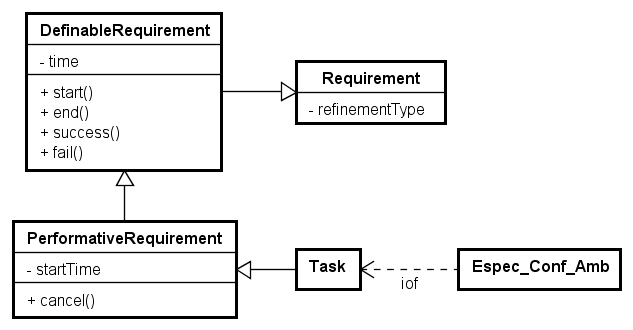
\includegraphics[width=1\textwidth]{figuras/exemplos-emf/exemplo-instanciacao-ecore.PNG}
	\caption{Exemplo de um elemento do modelo de domínio específico instanciado em \zanshin.}
	\label{exemplo-instanciacao-ecore}
\end{figure}

\textit{Performative Requirements} definem os tipos de requisitos que são ou podem ser refinados em tarefas, e assim possuem ações que são executadas pelo sistema ou seus usuários. \textit{Definable Requirements} são os requisitos que deve possuir um estado definido em algum momento da execução, como por exemplo os objetivos e pressuposições de domínio.

Assim que o \zanshin cria as classes dos requisitos do sistema alvo, o processo de monitoramento apoia nos métodos definidos nas metaclasses \texttt{DefinableRequirement} e \texttt{PerformativeRequirement}~\cite{tesevitor} para realizar a monitoração, os métodos disponíveis são:
\begin{itemize}
	\item \texttt{start()}: esse método é chamado nas classes de critérios de qualidade e pressuposições de domínio imediatamente antes da análise de seu estado de satisfação. Para o caso de tarefas, esse método é chamado assim que um usuário inicia uma tarefa, e então todos os ancestrais a esse elemento também tem esse método invocado.
	\item \texttt{sucess()}: chamado quando um requisito é satisfeito e propagado para todos os acentrais a esse objetivo para ``avisar'' que o filho chegou ao estado de sucesso.
	\item \texttt{fail()}: segue a mesma lógica dos item anteriores, propagando a ``falha'' de um requisito aos seus ancestrais.
	\item \texttt{cancel()}: para o caso de requisitos como objetivos e tarefas, esse método é usado quando um procedimento é cancelado pelo usuário, e usa da mesma lógica de propagação dos métodos anteriores para informar o ocorrido aos pais.
	\item \texttt{end()}: chamado assim que um requisito muda para os estados de sucesso, falha ou cancelamento.
\end{itemize}

Através da descrição dos métodos acima mencionados, é possível entender como o processo de monitoramento funciona: basicamente os requisitos monitorados possuem métodos que podem ser chamados em cada caso que assumem, seja de sucesso, falha o ou cancelamento. Assim que chamados, os métodos invocam os mesmos procedimentos nos elementos pais, permitindo que a atualização de um requisito se propague a todos os elementos que interessem, atualizando assim todo o modelo.

Logo que o componente monitor detecta uma mudança de estado em um requisito, ou seja, assim que qualquer um dos métodos acima é invocado, ele imediatamente envia uma notificação sobre essa mudança ao módulo de adaptação, que então inicia o processo definido para aquele determinado requisito de percepção ~\cite{tesevitor}.

\subsection{Adaptação}
\label{sec-referencial-zanshin-adaptacao}
Em termos de implementação, o algoritmo do módulo de adaptação cria uma sessão para cada \awreq que está sendo monitorado e então gera uma fila de eventos que se referem a estratégias adaptativas. Assim, essa linha de eventos pode ser usada para verificar se uma estratégia é ou não aplicável a determinada situação. Primeiramente, deve-se verificar o estado de um objetivo apontado por um \awreq, para isso é checada a condição de resolução daquele. Então, caso uma avaliação considere que o objetivo está em estado de falha, o sistema segue (seguindo uma ordem pré-definida) a lista de estratégias de adaptação disponíveis, procurando alguma que tenha sua condição de aplicabilidade verdadeira. Caso encontre, aplica a estratégia definida por aquela condição de aplicabilidade e então retorna ao estado inicial, onde a checagem da satisfabilidade do objetivo é realizada novamente. Caso o sistema retorne a fase de checagem do estado do objetivo e esse ainda não tenha sido satisfeito, o processo começa novamente, obedecendo restrições como o número de tentativas de aplicação de uma estratégia, definido individualmente. Caso não encontre uma condição para aplicar uma estratégia, o sistema ativa o método ``abortar'' (\texttt{abort()})~\cite{souza2013requirements}. 

Ao final, quando uma sessão de adaptação é considerada resolvida, a mesma deve ser terminada e se for necessário que o processo seja aplicado novamente, uma nova sessão é criada. Entretanto, se uma sessão termina sem ter resolvido o problema, o \textit{framework} continuará trabalhando nela do ponto em que parou assim que receber uma nova requisição para adaptação daquele mesmo \awreq. Porém, algumas estratégias também podem forçar que a sessão seja reiniciada quando executada ~\cite{souza2013requirements}. Essa processo é conhecido como Evento de Ação-Condição (\textit{Event Condition Action} ou \textit{ECA}) ~\cite{morin2009models}.

\subsubsection{ECA}
\label{sec-referencial-zanshin-eca}

O código mostrado em~\ref{codigo-eca} resume o processo \textit{ECA} para realizar a seleção de estratégias de adaptação:

\begin{lstlisting}[caption={Código do processo ECA},label={codigo-eca}]
processEvent(ar : AwReq) {
	session = findOrCreateSession(ar.class);
	session.addEvent(ar);
	solved = ar.condition.evaluate(session);
	if(solved) break;

	ar.selectedStrategy = null;
	for each s in ar.strategies {
		appl = s.condition.evaluate(session);
		if (appl) {
			ar.selectedStrategy = s;
			break ;
		}
	}

	if (ar.selectedStrategy == null)
		ar.selectedStrategy = ABORT;

	ar.selectedStrategy.execute(session);
	ar.condition.evaluate(session);
}
\end{lstlisting}

O algoritmo de~\ref{codigo-eca} incia obtendo a sessão de adaptação referente a classe do \awreq requisitado (caso não haja uma sessão, uma nova é criada). Obtida a sessão de adaptação, o algoritmo tem então acesso a lista de eventos de aplicabilidade referentes, então, adiciona o \awreq a sessão e imediatamente verifica o estado da mesma (verificando a condição de resolução), parando caso tenha retornado estado de sucesso. Caso contrário, o processo continua procurando por uma estratégia que seja aplicável, verificando se a condição de aplicabilidade é verdadeira; se sim, interrompe o processo e dá a sessão de adaptação uma nova chance de verificar o estado do \awreq. Caso todas as condições sejam falsas e nenhuma estratégia seja selecionada, seleciona a estratégia padrão (\texttt{abort()}) e termina o processo~\cite{tesevitor}. 

Para exemplificar esse processo, tomemos novamente o \awreq ``AR15'', que garante que o requisito ``Registrar chamada'' deve nunca falhar. Caso seja detectado pelo processo de monitoramento que esse requisito apresenta estado de falha, o módulo monitor imediatamente ativa o componente de adaptação, que segue o processo ECA para aplicar estratégias ao ``AR15''. Pela Listagem~\ref{listagem-estrategias-AR15}, ve-se que a condição de resolução desse requisito é do tipo \texttt{SimpleResolutionCondition} (solucionado se os filhos, dependendo do refinamento, estão solucionados), e que a primeira estratégia a ser selecionada é \texttt{RetryStrategy}, ou seja, tentar novamente (em 5s), entretanto essa estratégia possui a condição de aplicabilidade \texttt{MaxExecutionsPerSessionApplicabilityCondition}, o que significa que ela só pode ser aplicada um determinado número de vezes naquela sessão (nesse caso apenas uma vez, de acordo com o atributo \texttt{maxExecutions}). Caso essa condição seja falsa, a próxima estratégia refere-se a desativar um dos filhos desse objetivo (\texttt{RelaxDisableChildStrategy}), no caso a tarefa ``Detectar localização da chamada'', e possui a mesma condição de aplicabilidade. Se nenhuma dessas condições puder ser satisfeitas, então o sistema aborta, caso contrário, seleciona a primeira estratégia aplicável e verifica novamente o estado do objetivo. A condição \texttt{SimpleResolutionCondition} refere-se ao fato de que um objetivo é dito satisfeito apenas se seus filhos estiverem em estado de sucesso (respeitando a regra booleana do refinamento). 

\begin{lstlisting}[caption={Estratégias de adaptação de AR15},label={listagem-estrategias-AR15}]
<awreqs xsi:type="acad:AR15">										
	<condition xsi:type="eca:SimpleResolutionCondition"/>
		<strategies xsi:type="eca:RetryStrategy" time="5000">
			<condition xsi:type="eca:MaxExecutionsPerSessionApplicabilityCondition" maxExecutions="1"/>
		</strategies>
		<strategies xsi:type="eca:RelaxDisableChildStrategy" child="//@rootGoal/@refinements.0/@refinements.0/@refinements.1">
			<condition xsi:type="eca:MaxExecutionsPerSessionApplicabilityCondition" maxExecutions="1"/>
		</strategies>
</awreqs>
\end{lstlisting}

É importante salientar que as classes referentes a estratégias de adaptação, assim como as condições de aplicabilidade e resolução podem ser estendidas para casos mais complexos, envolvendo inclusive a interação humana ~\cite{tesevitor}. Uma lista completa das estratégias de adaptação disponíveis por padrão no \zanshin é mostrada na Tabela~\ref{awreqs-zanshin}.

\begin{table}[]
	\centering
	\caption{Tabela de Requisitos de Adaptação}
	\label{awreqs-zanshin}
	\begin{tabular}{|l|l|}
		\hline
		Regra                              & Efeito                                                                          \\ \hline
		Abort()                            & Sistema deve falhar de forma prevista, exibindo mensagem de falha, por exemplo. \\ \hline
		Delegate(a)                        & Delegar tarefa a um outro ator do sistema.                                      \\ \hline
		RelaxDisableChild(r, l, child)     & Para de considerar o estado de um requisito em determinada execução do sistema. \\ \hline
		Replace(r, copy, l, newReq)        & Substitui requisito.                                                            \\ \hline
		Retry(copy, time)                  & Tenta novamente em determinado período de tempo.                                \\ \hline
		StrengthenEnableChild(r, l, child) & Volta a considerar estado de um requisito.                                      \\ \hline
		Warning(a)                         & Avisa um ator sobre o estado atual do sistema.                                  \\ \hline
	\end{tabular}
\end{table}

%For example, the trivial case is considering the problem solved if the (next) AwReq evaluates to success, but this abstract class can be extended to provide di↵erent kinds of resolution conditions, including, e.g., involving a human-in-the-loop to confirm if the problem has indeed been solved, organizing conditions into AND/OR-refinement trees (like in a goal model), etc.

% ======================================================================================================
% SUBSEÇÃO DESENVOLVIMENTO ORIENTADO A MODELOS
% ======================================================================================================
\section{Desenvolvimento Orientado a Modelos}
\label{referencial-mdd}
Pesquisadores vem tentando ao longo dos anos criar abstrações que ajudem programadores a focar no conteúdo do desenvolvimento ao invés das especifidades da tecnologia de criação adotada~\cite{viyovic2014sirius}. O Desenvolvimento Orientado a Modelos  pode ser visto como a forma de programação de mais alto nível de abstração existente atualmente~\cite{atkinson2003model}, promovendo o uso de artefatos do processo de desenvolvimento de software para lidar com complexidade através de abstração~\cite{viyovic2014sirius}. Em outras palavras, MDD parte da premissa que um sistema é um modelo consistente com seu metamodelo~\cite{vujovic2014comparative} e assim, em vez de exigir que programadores escrevam cada simples detalhe da implementação de um sistema, permite que uma funcionalidade necessária para um software pode ser visualmente modelada ~\cite{atkinson2003model}. Portanto, essa técnica viabiliza que muitas atividades complexas (porém rotineiras) sejam automatizadas na área de programação de software, como por exemplo o suporte a persistência, interoperabilidade e distribuição ~\cite{atkinson2003model}.

A modelagem usa da percepção visual humana para melhorar o processo de compreensão sobre o domínio de um software, já que modelos nos auxiliam a entender problema complexos e suas possíveis soluções através da abstração. Assim, MDD baseia-se na premissa de que o desenvolvimento de software deve focar principalmente na produção de modelos e não na criação de código ~\cite{selic2003pragmatics}. A primeira vantagem dessa abordagem é que podemos usar conceitos mais ligados ao domínio do problema que software vai resolver do que conceitos técnicos ligados a linguagem de programação, em consequência essa vantagem acarreta em alguns outros benefícios: modelos são mais compreensíveis do que códigos e portanto, tornam-se também mais fáceis de especificar e manter~\cite{selic2003pragmatics}. Além disso, modelos são menos sensíveis a alterações de tecnologias, ou seja, são independentes de plataforma~\cite{selic2003pragmatics}. Esse trabalho foca em MDD como ferramente de produção automática de código através da interpretação de modelos visuais~\cite{selic2003pragmatics, viyovic2014sirius}.

\subsection{Eclipse Modeling Framework}
O \eclipse é um projeto de código aberto com o objetivo de prover uma plataforma de desenvolvimento altamente integrada. O processo de criação de sistemas no \eclipse pode ser divido em alguns projetos, entre eles o Projeto de Modelagem (\textit{Modeling Project}), que foca em tecnologias baseadas no desenvolvimento orientado a modelos~\cite{steinberg2008emf}. Esse ambiente é chamado de \textit{Eclipse Modeling Framework} ou \textit{EMF}, e provê funcionalidades como transformação de modelos, integração de bases de dados e geração de editores gráficos~\cite{steinberg2008emf}. Modelos especificados através de \emf relacionam abstrações de modelagem diretamente a seus conceitos de implementação, sendo a união das tecnologias \uml, \xml e \java, permitindo a conversão automática entre todas essas ferramentas~\cite{steinberg2008emf}. 

A tecnologia \emf pode ser melhor explicada com um exemplo: um sistema de gerenciamento de ordem de compras de uma loja, que necessite incluir casos como ``cobrar'' e ``entregar'' em um endereço, e uma coleção de itens (nesse caso compras). A figura~\ref{exemplo-uml} mostra o diagrama em \uml do sistema. Esse modelo pode também ser descrito dentro do \emf usando modelos \ecore, como na Figura~\ref{exemplo-ecore}. Modelos \ecore são basedos no metamodelo para especificação exibido na Figura~\ref{metamodelo-ecore}, onde classes são representadas por \texttt{EClass}, atributos por \texttt{EAttribute}, relações por \texttt{EReference} e tipos de dados por \texttt{EDataType}. Assim, a ``conversão'' do modelo \uml para \ecore é dada ao se instanciar classes de \ecore de acordo com a especificidade do domínio do problema, como pode ser visto na Figura~\ref{exemplo-uml-to-ecore}~\cite{steinberg2008emf}. 

\begin{figure}[h]
	\centering
	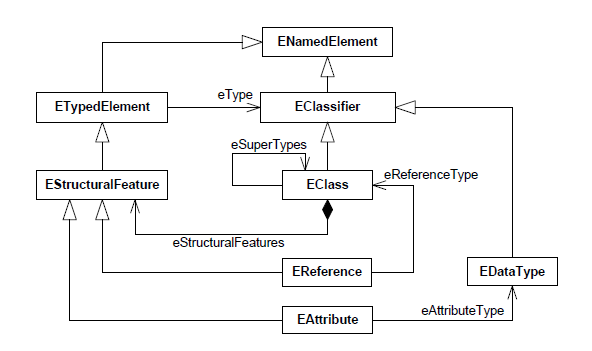
\includegraphics[width=0.95\textwidth]{figuras/exemplos-emf/metamodelo-ecore.png}
	\caption{Metamodelo de \ecore~\cite{kern2008interchange}}
	\label{metamodelo-ecore}
\end{figure}

\begin{figure}[h]
	\centering
	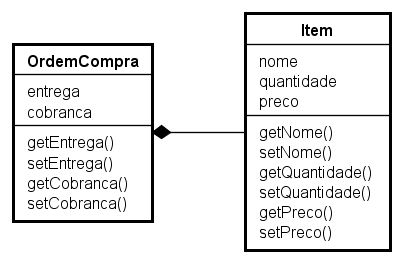
\includegraphics[width=0.65\textwidth]{figuras/exemplos-emf/exemplo-uml.png}
	\caption{Classes do diagrama do exemplo em \uml}
	\label{exemplo-uml}
\end{figure}

\begin{figure}[h]
	\centering
	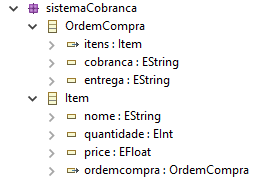
\includegraphics[width=0.7\textwidth]{figuras/exemplos-emf/exemplo-ecore.PNG}
	\caption{Classes do diagrama do exemplo em \ecore}
	\label{exemplo-ecore}
\end{figure}

Assim que o modelo é detalhado em \ecore, o \emf está pronto para gerar código automaticamente, seguindo os seguintes passos:

\begin{itemize}
	\item Para cada tipo \texttt{EClass} são criadas uma interface e a classe de implementação correspondente. Então para o exemplo de classe \texttt{OrdemCompra} serão criadas a interface \texttt{OrdemCompra} e a classe \texttt{OrdemCompraImpl}. Essa especificação permite que sejam implementadas funções de persistência e distribuição, porém não serão discutidas aqui por fugirem do escopo desse trabalho.
	\item As classes do tipo \texttt{EAtributte} são transformadas em atributos nas classes correspondentes
	\item As classes tipo \texttt{EReference} são transformadas em referências nas respectivas classes as quais referenciam.
\end{itemize}

\begin{figure}[h]
	\centering
	
\includegraphics[width=1\textwidth]{figuras/exemplos-emf/uml-to-ecore.png}
	\caption{Conversão do diagrama de exemplo de \uml para \ecore}
	\label{exemplo-uml-to-ecore}
\end{figure}

Em suma, o \framework de modelagem do \eclipse permite que usuários criem modelos apoiados em metamodelos, e baseando-se no modelo criado, gerem partes de código de sistema~\cite{vujovic2014comparative}.

%https://books.google.com.br/books?id=sA0zOZuDXhgC&lpg=PT23&ots=2IQIWZWqNm&dq=eclipse&lr&hl=pt-BR&pg=PT45#v=onepage&q=eclipse&f=false

\subsection{Sirius}

O \sirius é um plugin que simplifica o \framework de Modelagem Gráfica (\textit{Graphical Modeling Framework} ou \textit{GMF}) do \eclipse, reduzindo a complexidade de uso do mesmo e permitindo a produção de editores gráficos de modelos personalizados~\cite{viyovic2014sirius}. O \sirius é construído em cima do fato de que o \eclipse provê utilidades para (des)serialização de modelos, checagem de condições e geração de editores baseados em \ecore~\cite{budinsky2004eclipse}. Representações criadas com \sirius podem ser apresentadas em diagramas, tabelas e árvores~\cite{viyovic2014sirius}. Em síntese, \sirius provê ferramentas que permitem a especificação de um modelo de um domínio qualquer em diferentes perspectivas gráficas~\cite{vujovic2014comparative}.

Através de modelos de especificação (\textit{Viewpoint Specification Model} ou VSM), o \textit{plugin} permite especificar a estrutura, aparência e comportamento do metamodelo do editor a ser criado~\cite{viyovic2014sirius}. Os VSMs são especificados através de arquivos \textit{.odesign}~\cite{viyovic2014sirius}, e baseam-se metamodelo de domínio descrito em \ecore. Um exemplo de caracterização de representação de modelos é mostrado na figura~\ref{exemplo-sirius}.

\begin{figure}[h]
	\centering
	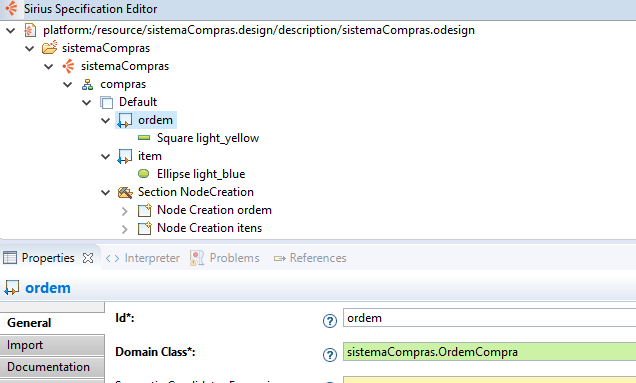
\includegraphics[width=0.9\textwidth]{figuras/exemplos-emf/exemplo-sirius-vsm.png}
	\caption{Exemplo de \textit{Viewpoint Specification Model}}
	\label{exemplo-sirius}
\end{figure}

\sirius provê vários mecanismos que auxiliam no gerenciamento da complexidade de modelos~\cite{madiot2015eclipse}:

\begin{itemize}
	\item \textbf{Camadas}: é possível separar elementos em camadas diferentes, e ativar ou desativar essas.
	\item \textbf{Filtros}: exibir ou esconder elementos dependendo de determinada condição.
	\item \textbf{Fersonalização de Estilos}: permite modificar propriedades gráficas de elementos do diagrama.
	\item \textbf{Regras de Validação}: permite que a qualidade do modelo seja avaliada.
\end{itemize}

